\documentclass[]{article}
\usepackage{lmodern}
\usepackage{amssymb,amsmath}
\usepackage{ifxetex,ifluatex}
\usepackage{fixltx2e} % provides \textsubscript
\ifnum 0\ifxetex 1\fi\ifluatex 1\fi=0 % if pdftex
  \usepackage[T1]{fontenc}
  \usepackage[utf8]{inputenc}
\else % if luatex or xelatex
  \ifxetex
    \usepackage{mathspec}
  \else
    \usepackage{fontspec}
  \fi
  \defaultfontfeatures{Ligatures=TeX,Scale=MatchLowercase}
\fi
% use upquote if available, for straight quotes in verbatim environments
\IfFileExists{upquote.sty}{\usepackage{upquote}}{}
% use microtype if available
\IfFileExists{microtype.sty}{%
\usepackage{microtype}
\UseMicrotypeSet[protrusion]{basicmath} % disable protrusion for tt fonts
}{}
\usepackage[margin=1in]{geometry}
\usepackage{hyperref}
\hypersetup{unicode=true,
            pdftitle={Caravan Insurance Challenge},
            pdfauthor={Yash},
            pdfborder={0 0 0},
            breaklinks=true}
\urlstyle{same}  % don't use monospace font for urls
\usepackage{color}
\usepackage{fancyvrb}
\newcommand{\VerbBar}{|}
\newcommand{\VERB}{\Verb[commandchars=\\\{\}]}
\DefineVerbatimEnvironment{Highlighting}{Verbatim}{commandchars=\\\{\}}
% Add ',fontsize=\small' for more characters per line
\usepackage{framed}
\definecolor{shadecolor}{RGB}{248,248,248}
\newenvironment{Shaded}{\begin{snugshade}}{\end{snugshade}}
\newcommand{\KeywordTok}[1]{\textcolor[rgb]{0.13,0.29,0.53}{\textbf{#1}}}
\newcommand{\DataTypeTok}[1]{\textcolor[rgb]{0.13,0.29,0.53}{#1}}
\newcommand{\DecValTok}[1]{\textcolor[rgb]{0.00,0.00,0.81}{#1}}
\newcommand{\BaseNTok}[1]{\textcolor[rgb]{0.00,0.00,0.81}{#1}}
\newcommand{\FloatTok}[1]{\textcolor[rgb]{0.00,0.00,0.81}{#1}}
\newcommand{\ConstantTok}[1]{\textcolor[rgb]{0.00,0.00,0.00}{#1}}
\newcommand{\CharTok}[1]{\textcolor[rgb]{0.31,0.60,0.02}{#1}}
\newcommand{\SpecialCharTok}[1]{\textcolor[rgb]{0.00,0.00,0.00}{#1}}
\newcommand{\StringTok}[1]{\textcolor[rgb]{0.31,0.60,0.02}{#1}}
\newcommand{\VerbatimStringTok}[1]{\textcolor[rgb]{0.31,0.60,0.02}{#1}}
\newcommand{\SpecialStringTok}[1]{\textcolor[rgb]{0.31,0.60,0.02}{#1}}
\newcommand{\ImportTok}[1]{#1}
\newcommand{\CommentTok}[1]{\textcolor[rgb]{0.56,0.35,0.01}{\textit{#1}}}
\newcommand{\DocumentationTok}[1]{\textcolor[rgb]{0.56,0.35,0.01}{\textbf{\textit{#1}}}}
\newcommand{\AnnotationTok}[1]{\textcolor[rgb]{0.56,0.35,0.01}{\textbf{\textit{#1}}}}
\newcommand{\CommentVarTok}[1]{\textcolor[rgb]{0.56,0.35,0.01}{\textbf{\textit{#1}}}}
\newcommand{\OtherTok}[1]{\textcolor[rgb]{0.56,0.35,0.01}{#1}}
\newcommand{\FunctionTok}[1]{\textcolor[rgb]{0.00,0.00,0.00}{#1}}
\newcommand{\VariableTok}[1]{\textcolor[rgb]{0.00,0.00,0.00}{#1}}
\newcommand{\ControlFlowTok}[1]{\textcolor[rgb]{0.13,0.29,0.53}{\textbf{#1}}}
\newcommand{\OperatorTok}[1]{\textcolor[rgb]{0.81,0.36,0.00}{\textbf{#1}}}
\newcommand{\BuiltInTok}[1]{#1}
\newcommand{\ExtensionTok}[1]{#1}
\newcommand{\PreprocessorTok}[1]{\textcolor[rgb]{0.56,0.35,0.01}{\textit{#1}}}
\newcommand{\AttributeTok}[1]{\textcolor[rgb]{0.77,0.63,0.00}{#1}}
\newcommand{\RegionMarkerTok}[1]{#1}
\newcommand{\InformationTok}[1]{\textcolor[rgb]{0.56,0.35,0.01}{\textbf{\textit{#1}}}}
\newcommand{\WarningTok}[1]{\textcolor[rgb]{0.56,0.35,0.01}{\textbf{\textit{#1}}}}
\newcommand{\AlertTok}[1]{\textcolor[rgb]{0.94,0.16,0.16}{#1}}
\newcommand{\ErrorTok}[1]{\textcolor[rgb]{0.64,0.00,0.00}{\textbf{#1}}}
\newcommand{\NormalTok}[1]{#1}
\usepackage{graphicx,grffile}
\makeatletter
\def\maxwidth{\ifdim\Gin@nat@width>\linewidth\linewidth\else\Gin@nat@width\fi}
\def\maxheight{\ifdim\Gin@nat@height>\textheight\textheight\else\Gin@nat@height\fi}
\makeatother
% Scale images if necessary, so that they will not overflow the page
% margins by default, and it is still possible to overwrite the defaults
% using explicit options in \includegraphics[width, height, ...]{}
\setkeys{Gin}{width=\maxwidth,height=\maxheight,keepaspectratio}
\IfFileExists{parskip.sty}{%
\usepackage{parskip}
}{% else
\setlength{\parindent}{0pt}
\setlength{\parskip}{6pt plus 2pt minus 1pt}
}
\setlength{\emergencystretch}{3em}  % prevent overfull lines
\providecommand{\tightlist}{%
  \setlength{\itemsep}{0pt}\setlength{\parskip}{0pt}}
\setcounter{secnumdepth}{0}
% Redefines (sub)paragraphs to behave more like sections
\ifx\paragraph\undefined\else
\let\oldparagraph\paragraph
\renewcommand{\paragraph}[1]{\oldparagraph{#1}\mbox{}}
\fi
\ifx\subparagraph\undefined\else
\let\oldsubparagraph\subparagraph
\renewcommand{\subparagraph}[1]{\oldsubparagraph{#1}\mbox{}}
\fi

%%% Use protect on footnotes to avoid problems with footnotes in titles
\let\rmarkdownfootnote\footnote%
\def\footnote{\protect\rmarkdownfootnote}

%%% Change title format to be more compact
\usepackage{titling}

% Create subtitle command for use in maketitle
\newcommand{\subtitle}[1]{
  \posttitle{
    \begin{center}\large#1\end{center}
    }
}

\setlength{\droptitle}{-2em}

  \title{Caravan Insurance Challenge}
    \pretitle{\vspace{\droptitle}\centering\huge}
  \posttitle{\par}
    \author{Yash}
    \preauthor{\centering\large\emph}
  \postauthor{\par}
      \predate{\centering\large\emph}
  \postdate{\par}
    \date{June 24, 2018}


\begin{document}
\maketitle

\section{Predicting Caravan Insurance
Purchases}\label{predicting-caravan-insurance-purchases}

\subsection{The data is provided by the Caravan Insurance company of its
customer base. Some of the customers have already bought policies for
fire risk , auto , boat etc from Caravan. Using this information we need
predict whether they will purchase Caravan Home
Insurance}\label{the-data-is-provided-by-the-caravan-insurance-company-of-its-customer-base.-some-of-the-customers-have-already-bought-policies-for-fire-risk-auto-boat-etc-from-caravan.-using-this-information-we-need-predict-whether-they-will-purchase-caravan-home-insurance}

\subsection{This is a classification problem. It is a high dimension
dataset with 86 variables. The number of people who have bought
insurance is very low, less than 5\%. We will use tree based methods
like Random forest and Boosted trees to
predict.}\label{this-is-a-classification-problem.-it-is-a-high-dimension-dataset-with-86-variables.-the-number-of-people-who-have-bought-insurance-is-very-low-less-than-5.-we-will-use-tree-based-methods-like-random-forest-and-boosted-trees-to-predict.}

\subsubsection{Load the training data and inspect the
data}\label{load-the-training-data-and-inspect-the-data}

\begin{Shaded}
\begin{Highlighting}[]
\NormalTok{Cins <-}\StringTok{  }\KeywordTok{read.csv.sql}\NormalTok{(}\StringTok{"C1.csv"}\NormalTok{,}\StringTok{"select * from file where ORIGIN = 'train' "}\NormalTok{, }\DataTypeTok{header=}\OtherTok{TRUE}\NormalTok{, }\DataTypeTok{sep=}\StringTok{","}\NormalTok{)}

\NormalTok{### Exclude the  first column }
\NormalTok{Caravan_train <-}\StringTok{ }\NormalTok{Cins[}\OperatorTok{-}\DecValTok{1}\NormalTok{]}


\NormalTok{### Check the dimensions}
\KeywordTok{dim}\NormalTok{(Caravan_train )}
\end{Highlighting}
\end{Shaded}

\begin{verbatim}
## [1] 5822   86
\end{verbatim}

\begin{Shaded}
\begin{Highlighting}[]
\CommentTok{#names(Caravan_train )}


\CommentTok{# Inspect the data }
\KeywordTok{str}\NormalTok{(Caravan_train )}
\end{Highlighting}
\end{Shaded}

\begin{verbatim}
## 'data.frame':    5822 obs. of  86 variables:
##  $ Customer_Subtype                             : int  33 37 37 9 40 23 39 33 33 11 ...
##  $ Number_of_houses                             : int  1 1 1 1 1 1 2 1 1 2 ...
##  $ Avg_size_household                           : int  3 2 2 3 4 2 3 2 2 3 ...
##  $ Avg_age                                      : int  2 2 2 3 2 1 2 3 4 3 ...
##  $ Customer_main_type                           : int  8 8 8 3 10 5 9 8 8 3 ...
##  $ Roman_catholic                               : int  0 1 0 2 1 0 2 0 0 3 ...
##  $ Protestant                                   : int  5 4 4 3 4 5 2 7 1 5 ...
##  $ Other_religion                               : int  1 1 2 2 1 0 0 0 3 0 ...
##  $ No_religion                                  : int  3 4 4 4 4 5 5 2 6 2 ...
##  $ Married                                      : int  7 6 3 5 7 0 7 7 6 7 ...
##  $ Living_together                              : int  0 2 2 2 1 6 2 2 0 0 ...
##  $ Other_relation                               : int  2 2 4 2 2 3 0 0 3 2 ...
##  $ Singles                                      : int  1 0 4 2 2 3 0 0 3 2 ...
##  $ Household_without_children                   : int  2 4 4 3 4 5 3 5 3 2 ...
##  $ Household_with_children                      : int  6 5 2 4 4 2 6 4 3 6 ...
##  $ High_level_education                         : int  1 0 0 3 5 0 0 0 0 0 ...
##  $ Medium_level_education                       : int  2 5 5 4 4 5 4 3 1 4 ...
##  $ Lower_level_education                        : int  7 4 4 2 0 4 5 6 8 5 ...
##  $ High_status                                  : int  1 0 0 4 0 2 0 2 1 2 ...
##  $ Entrepreneur                                 : int  0 0 0 0 5 0 0 0 1 0 ...
##  $ Farmer                                       : int  1 0 0 0 4 0 0 0 0 0 ...
##  $ Middle_management                            : int  2 5 7 3 0 4 4 2 1 3 ...
##  $ Skilled_labourers                            : int  5 0 0 1 0 2 1 5 8 3 ...
##  $ Unskilled_labourers                          : int  2 4 2 2 0 2 5 2 1 3 ...
##  $ Social_class_A                               : int  1 0 0 3 9 2 0 2 1 1 ...
##  $ Social_class_B1                              : int  1 2 5 2 0 2 1 1 1 2 ...
##  $ Social_class_B2                              : int  2 3 0 1 0 2 4 2 0 1 ...
##  $ Social_class_C                               : int  6 5 4 4 0 4 5 5 8 4 ...
##  $ Social_class_D                               : int  1 0 0 0 0 2 0 2 1 2 ...
##  $ Rented_house                                 : int  1 2 7 5 4 9 6 0 9 0 ...
##  $ Home_owners                                  : int  8 7 2 4 5 0 3 9 0 9 ...
##  $ X1_car                                       : int  8 7 7 9 6 5 8 4 5 6 ...
##  $ X2_cars                                      : int  0 1 0 0 2 3 0 4 2 1 ...
##  $ No_car                                       : int  1 2 2 0 1 3 1 2 3 2 ...
##  $ National_Health_Service                      : int  8 6 9 7 5 9 9 6 7 6 ...
##  $ Private_health_insurance                     : int  1 3 0 2 4 0 0 3 2 3 ...
##  $ Income_._30                                  : int  0 2 4 1 0 5 4 2 7 2 ...
##  $ Income_30.45.000                             : int  4 0 5 5 0 2 3 5 2 3 ...
##  $ Income_45.75.000                             : int  5 5 0 3 9 3 3 3 1 3 ...
##  $ Income_75.122.000                            : int  0 2 0 0 0 0 0 0 0 1 ...
##  $ Income_.123.000                              : int  0 0 0 0 0 0 0 0 0 0 ...
##  $ Average_income                               : int  4 5 3 4 6 3 3 3 2 4 ...
##  $ Purchasing_power                             : int  3 4 4 4 3 3 5 3 3 7 ...
##  $ private_third_party_insurance                : int  0 2 2 0 0 0 0 0 0 2 ...
##  $ third_party_insurance_firms                  : int  0 0 0 0 0 0 0 0 0 0 ...
##  $ third_party_insurane_agriculture             : int  0 0 0 0 0 0 0 0 0 0 ...
##  $ car_policies                                 : int  6 0 6 6 0 6 6 0 5 0 ...
##  $ delivery_van_policies                        : int  0 0 0 0 0 0 0 0 0 0 ...
##  $ Contribution_motorcycle_scooter              : int  0 0 0 0 0 0 0 0 0 0 ...
##  $ lorry_policies                               : int  0 0 0 0 0 0 0 0 0 0 ...
##  $ trailer_policies                             : int  0 0 0 0 0 0 0 0 0 0 ...
##  $ tractor_policies                             : int  0 0 0 0 0 0 0 0 0 0 ...
##  $ agricultural_machines_policies               : int  0 0 0 0 0 0 0 0 0 0 ...
##  $ moped_policies                               : int  0 0 0 0 0 0 0 3 0 0 ...
##  $ life_insurances                              : int  0 0 0 0 0 0 0 0 0 0 ...
##  $ private_accident_insurance_policies          : int  0 0 0 0 0 0 0 0 0 0 ...
##  $ family_accidents_insurance_policies          : int  0 0 0 0 0 0 0 0 0 0 ...
##  $ disability_insurance_policies                : int  0 0 0 0 0 0 0 0 0 0 ...
##  $ fire_policies                                : int  5 2 2 2 6 0 0 0 0 3 ...
##  $ surfboard_policies                           : int  0 0 0 0 0 0 0 0 0 0 ...
##  $ boat_policies                                : int  0 0 0 0 0 0 0 0 0 0 ...
##  $ bicycle_policies                             : int  0 0 0 0 0 0 0 0 0 0 ...
##  $ property_insurance_policies                  : int  0 0 0 0 0 0 0 0 0 0 ...
##  $ social_security_insurance_policies           : int  0 0 0 0 0 0 0 0 0 0 ...
##  $ Number_of_private_third_party_insurance      : int  0 2 1 0 0 0 0 0 0 1 ...
##  $ Number_of_third_party_insurance_firms        : int  0 0 0 0 0 0 0 0 0 0 ...
##  $ Number_of_third_party_insurane_agriculture   : int  0 0 0 0 0 0 0 0 0 0 ...
##  $ Number_of_car_policies                       : int  1 0 1 1 0 1 1 0 1 0 ...
##  $ Number_of_delivery_van_policies              : int  0 0 0 0 0 0 0 0 0 0 ...
##  $ Number_of_motorcycle_scooter_policies        : int  0 0 0 0 0 0 0 0 0 0 ...
##  $ Number_of_lorry_policies                     : int  0 0 0 0 0 0 0 0 0 0 ...
##  $ Number_of_trailer_policies                   : int  0 0 0 0 0 0 0 0 0 0 ...
##  $ Number_of_tractor_policies                   : int  0 0 0 0 0 0 0 0 0 0 ...
##  $ Number_of_agricultural_machines_policies     : int  0 0 0 0 0 0 0 0 0 0 ...
##  $ Number_of_moped_policies                     : int  0 0 0 0 0 0 0 1 0 0 ...
##  $ Number_of_life_insurances                    : int  0 0 0 0 0 0 0 0 0 0 ...
##  $ Number_of_private_accident_insurance_policies: int  0 0 0 0 0 0 0 0 0 0 ...
##  $ Number_of_family_accidents_insurance_policies: int  0 0 0 0 0 0 0 0 0 0 ...
##  $ Number_of_disability_insurance_policies      : int  0 0 0 0 0 0 0 0 0 0 ...
##  $ Number_of_fire_policies                      : int  1 1 1 1 1 0 0 0 0 1 ...
##  $ Number_of_surfboard_policies                 : int  0 0 0 0 0 0 0 0 0 0 ...
##  $ Number_of_boat_policies                      : int  0 0 0 0 0 0 0 0 0 0 ...
##  $ Number_of_bicycle_policies                   : int  0 0 0 0 0 0 0 0 0 0 ...
##  $ Number_of_property_insurance_policies        : int  0 0 0 0 0 0 0 0 0 0 ...
##  $ Number_of_social_security_insurance_policies : int  0 0 0 0 0 0 0 0 0 0 ...
##  $ Number_of_mobile_home_policies               : int  0 0 0 0 0 0 0 0 0 0 ...
\end{verbatim}

\begin{Shaded}
\begin{Highlighting}[]
\CommentTok{#head(Caravan_train )}
\end{Highlighting}
\end{Shaded}

\subsubsection{check for missing values}\label{check-for-missing-values}

\begin{Shaded}
\begin{Highlighting}[]
\NormalTok{Missing_Count <-}\StringTok{  }\KeywordTok{sum}\NormalTok{(}\KeywordTok{is.na.data.frame}\NormalTok{(Caravan_train))}
\KeywordTok{print}\NormalTok{(}\KeywordTok{paste}\NormalTok{ (}\StringTok{"Missing count -> "}\NormalTok{ , Missing_Count))}
\end{Highlighting}
\end{Shaded}

\begin{verbatim}
## [1] "Missing count ->  0"
\end{verbatim}

\subsubsection{Its an highly unbalanced dataset. This is evident from
the below bar
chart}\label{its-an-highly-unbalanced-dataset.-this-is-evident-from-the-below-bar-chart}

\begin{Shaded}
\begin{Highlighting}[]
\NormalTok{bar_label <-}\StringTok{ }\KeywordTok{factor}\NormalTok{(Caravan_train}\OperatorTok{$}\NormalTok{Number_of_mobile_home_policies  , }\DataTypeTok{labels=}\KeywordTok{c}\NormalTok{(}\StringTok{"NotPurchased"}\NormalTok{,}\StringTok{"Purchased"}\NormalTok{))}
\CommentTok{#bar_label}
\KeywordTok{ggplot}\NormalTok{(}\DataTypeTok{data =}\NormalTok{  Caravan_train, }\KeywordTok{aes}\NormalTok{(}\DataTypeTok{y =} \StringTok{""}\NormalTok{, }\DataTypeTok{x =}\NormalTok{Number_of_mobile_home_policies , }\DataTypeTok{fill =}\NormalTok{ bar_label ) )}\OperatorTok{+}\StringTok{ }
\StringTok{  }\KeywordTok{geom_bar}\NormalTok{(}\DataTypeTok{stat =} \StringTok{"identity"}\NormalTok{ ) }\OperatorTok{+}\StringTok{ }
\StringTok{  }\KeywordTok{ggtitle}\NormalTok{(}\StringTok{"Not Purchased /  Purchased"}\NormalTok{)}
\end{Highlighting}
\end{Shaded}

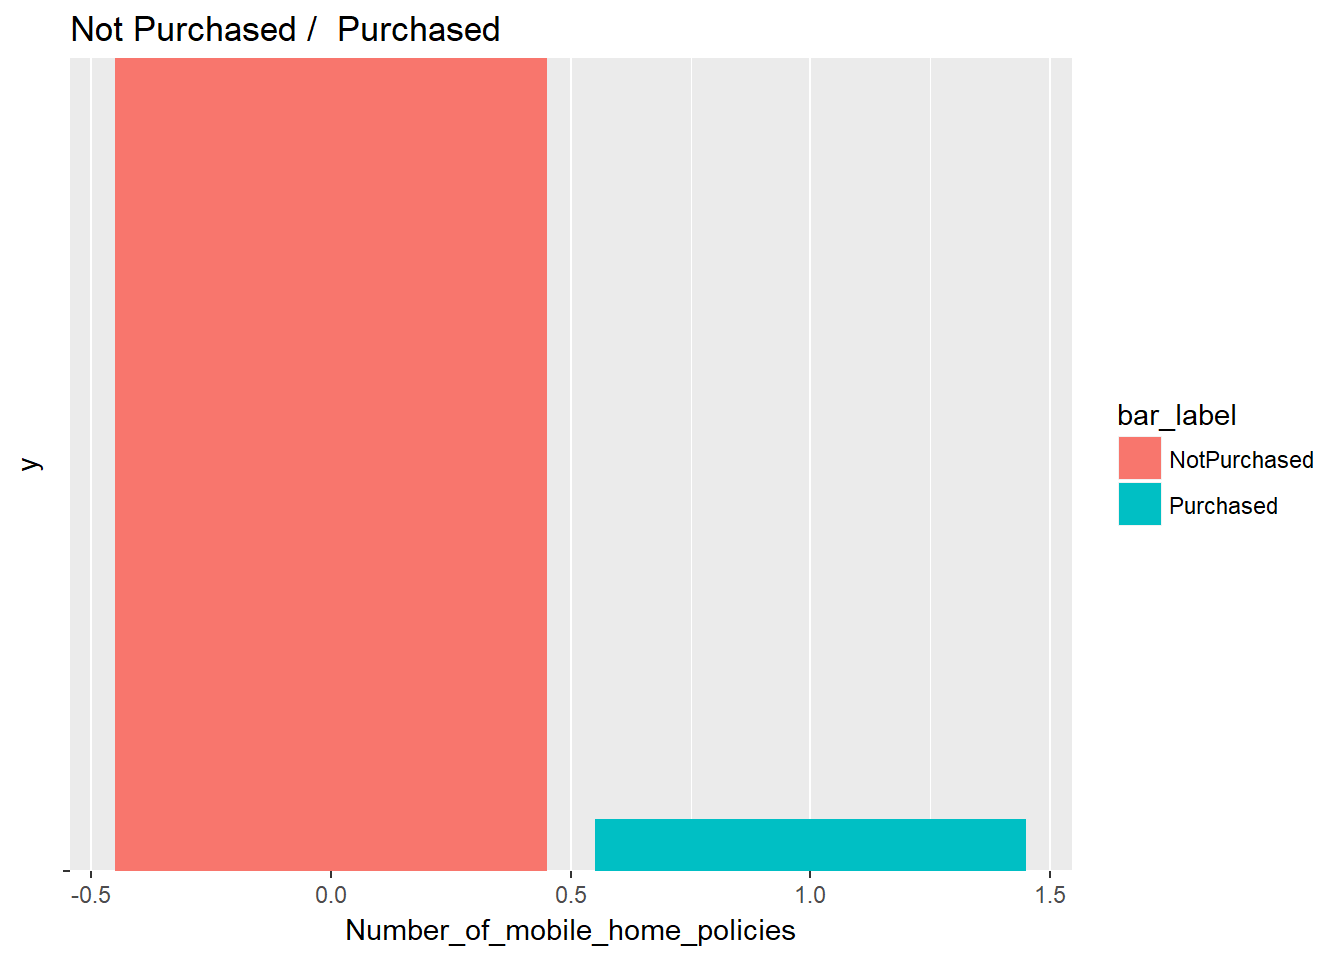
\includegraphics{CAPSTONE_RMD_files/figure-latex/unnamed-chunk-3-1.pdf}

\begin{Shaded}
\begin{Highlighting}[]
\KeywordTok{print}\NormalTok{(}\KeywordTok{paste}\NormalTok{(}\StringTok{"Insurance count : 0 -> not having insurance , 1 - Having Insurance"}\NormalTok{))}
\end{Highlighting}
\end{Shaded}

\begin{verbatim}
## [1] "Insurance count : 0 -> not having insurance , 1 - Having Insurance"
\end{verbatim}

\begin{Shaded}
\begin{Highlighting}[]
\KeywordTok{table}\NormalTok{(Caravan_train}\OperatorTok{$}\NormalTok{Number_of_mobile_home_policies)}
\end{Highlighting}
\end{Shaded}

\begin{verbatim}
## 
##    0    1 
## 5474  348
\end{verbatim}

\subsubsection{From the GBM variance influence chart, we will select
only 56 variables that have
impact}\label{from-the-gbm-variance-influence-chart-we-will-select-only-56-variables-that-have-impact}


\end{document}
